%----------------------------------------------------------------------------------------
%   Доорх хэсгийг өөрчлөх шаардлагагүй
%----------------------------------------------------------------------------------------
%!TEX TS-program = xelatex
%!TEX encoding = UTF-8 Unicode
\documentclass[12pt,A4]{report}

\usepackage{fontspec,xltxtra,xunicode}
\setmainfont[Ligatures=TeX]{Times New Roman}
\setsansfont{Arial}

% \usepackage[utf8x]{inputenc}
% \usepackage[mongolian]{babel}
%\usepackage{natbib}
\usepackage{geometry}
%\usepackage{fancyheadings} fancyheadings is obsolete: replaced by fancyhdr. JL
\usepackage{fancyhdr}
\usepackage{float}
\usepackage{afterpage}
\usepackage{graphicx}
\usepackage{amsmath,amssymb,amsbsy}
\usepackage{dcolumn,array}
\usepackage{tocloft}
\usepackage{dics}
\usepackage{nomencl}
\usepackage{upgreek}
\newcommand{\argmin}{\arg\!\min}
\usepackage{mathtools}
\usepackage[hidelinks]{hyperref}
\usepackage{bookmark}

\usepackage{algorithm}
\usepackage{algpseudocode}

\usepackage{listings}
\DeclarePairedDelimiter\abs{\lvert}{\rvert}%
\makeatletter
\usepackage{caption}
\captionsetup[table]{belowskip=0.5pt}
\usepackage{subfiles}

\usepackage{listings}
\renewcommand{\lstlistingname}{Код}
\renewcommand{\lstlistlistingname}{\lstlistingname ын жагсаалт}

\usepackage{color}
\definecolor{codegreen}{rgb}{0,0.6,0}
\definecolor{codegray}{rgb}{0.5,0.5,0.5}
\definecolor{codepurple}{rgb}{0.58,0,0.82}
\definecolor{backcolour}{rgb}{0.99,0.99,0.99}
\definecolor{darkgray}{rgb}{0.99,0.103,0.105}
\definecolor{purple}{rgb}{0.128,0,0.128}
 
\lstdefinestyle{mystyle}{
    basicstyle=\ttfamily\small,
    backgroundcolor=\color{backcolour},   
    commentstyle=\color{codegreen},
    keywordstyle=\color{magenta},
    numberstyle=\tiny\color{codegray},
    stringstyle=\color{codepurple},
    %basicstyle=\footnotesize,
    breakatwhitespace=false,         
    breaklines=true,                 
    captionpos=b,                    
    keepspaces=false,                 
    numbers=left,                    
    numbersep=10pt,                  
    showspaces=false,                
    showstringspaces=true,
    showtabs=false,                  
    tabsize=2
}
 
 %define Javascript language
\lstdefinelanguage{JavaScript}{
keywords={typeof, new, true, false, catch, function, return, null, catch, switch, var, if, in, while, do, else, case, break},
keywordstyle=\color{blue}\bfseries,
ndkeywords={class, export, boolean, throw, implements, import, this},
ndkeywordstyle=\color{darkgray}\bfseries,
identifierstyle=\color{black},
sensitive=false,
comment=[l]{//},
morecomment=[s]{/*}{*/},
commentstyle=\color{purple}\ttfamily,
stringstyle=\color{red}\ttfamily,
morestring=[b]',
morestring=[b]"
}
 
\lstset{
language=JavaScript,
extendedchars=true,
basicstyle=\footnotesize\ttfamily,
showstringspaces=false,
showspaces=false,
numbers=left,
numberstyle=\footnotesize,
numbersep=9pt,
tabsize=2,
breaklines=true,
showtabs=false,
captionpos=b
}
 
\lstset{style=mystyle, label=DescriptiveLabel} 


\let\oldabs\abs
\def\abs{\@ifstar{\oldabs}{\oldabs*}}
\makenomenclature
\begin{document}


%----------------------------------------------------------------------------------------
%   Өөрийн мэдээллээ оруулах хэсэг
%----------------------------------------------------------------------------------------

% Дипломийн ажлын сэдэв
\title{Зайнаас удирдах Веб хөтөч}
% Дипломын ажлын англи нэр
\titleEng{Remote access and remote control Web browser}
% Өөрийн овог нэрийг бүтнээр нь бичнэ
\author{Даваадорж Энхманлай}
% Өөрийн овгийн эхний үсэг нэрээ бичнэ
\authorShort{Д.Энхманлай}
% Удирдагчийн зэрэг цол овгийн эхний үсэг нэр
\supervisor{Г.Гантулга}
% Хамтарсан удирдагчийн зэрэг цол овгийн эхний үсэг нэр
%\cosupervisor{Ч.Алтангэрэл}

% СиСи дугаар 
\sisiId{20B1NUM0690}
% Их сургуулийн нэр
\university{МОНГОЛ УЛСЫН ИХ СУРГУУЛЬ}
% Бүрэлдэхүүн сургуулийн нэр
\faculty{МЭДЭЭЛЛИЙН ТЕХНОЛОГИ, ЭЛЕКТРОНИКИЙН СУРГУУЛЬ}
% Тэнхимийн нэр
\department{МЭДЭЭЛЭЛ, КОМПЬЮТЕРИЙН УХААНЫ ТЭНХИМ}
% Зэргийн нэр
\degreeName{Бакалаврын судалгааны ажил}
% Суралцаж буй хөтөлбөрийн нэр
\programeName{Мэдээллийн технологи(D061303)}
% Хэвлэгдсэн газар
\cityName{Улаанбаатар}
% Хэвлэгдсэн огноо
\gradyear{2024 оны 5 сар}


%----------------------------------------------------------------------------------------
%   Доорх хэсгийг өөрчлөх шаардлагагүй
%----------------------------------------------------------------------------------------
%----------------------Нүүр хуудастай хамаатай зүйлс----------------------------
\pagenumbering{roman}
\makefrontpage
\maketitle
\doublespace

% Decleration
\begin{huge}
\textbf{Зохиогчийн баталгаа}
\end{huge} \\ \ \\ 
\doublespace
Миний бие \@author \ "\@title" \ сэдэвтэй судалгааны ажлыг гүйцэтгэсэн болохыг зарлаж дараах зүйлсийг баталж байна:
\begin{itemize}
\item Ажил нь бүхэлдээ эсвэл ихэнхдээ Монгол Улсын Их Сургуулийн зэрэг горилохоор дэвшүүлсэн болно.
\item Энэ ажлын аль нэг хэсгийг эсвэл бүхлээр нь ямар нэг их, дээд сургуулийн зэрэг горилохоор оруулж байгаагүй.
\item Бусдын хийсэн ажлаас хуулбарлаагүй, ашигласан бол ишлэл, зүүлт хийсэн.
\item Ажлыг би өөрөө (хамтарч) хийсэн ба миний хийсэн ажил, үзүүлсэн дэмжлэгийг Бакалаврын судалгааны ажилд тодорхой тусгасан. 
\item Ажилд тусалсан бүх эх сурвалжид талархаж байна. 
\end{itemize} 
\ 

Гарын үсэг: \underline{\hspace{5cm}}

Огноо: 	\ \ \underline{\hspace{3cm}}

% Гарчгийг автоматаар оруулна
\setcounter{tocdepth}{1}
\tableofcontents

% Зургийн жагсаалтыг автоматаар оруулна
\listoffigures

% Хүснэгтийн жагсаалтыг автоматаар оруулна
\listoftables

% Кодын жагсаалтыг автоматаар оруулна

% This puts the word "Page" right justified above everything else.
\newpage
%% \addtocontents{lof}{Зураг~\hfill Хуудас \par}
\newpage
%% \addtocontents{lot}{Хүснэгт~\hfill Хуудас \par}

\renewcommand{\cftlabel}{Зураг}


\doublespace
\pagenumbering{arabic}


\begin{abstract}
	Миний бие Д.Энхманлай нь Бакалаврын судалгааны ажлын хугацаанд Network, Linux, File server, Remote Control,Web browser гэсэн технологиуд дээр голчлон ажилласан ба уг технологиуд ямар шалтгаанаар үүссэн, цаана нь технологийн ямар дэвшил, хөгжүүлэлтийн арга барил ашигладаг, компаниуд хэрхэн үүн дээр хөгжүүлэлт хийж эцсийн бүтээгдэхүүнийг гаргадаг, Мөн Монголын №1 оператор компани болох "Mobicom corporation llc" дэмжлэгтэйгээр Бакалаврын судалгааны ажлыг хийж гүйцэтгэлээ.
  
  \quad \quad \textbf{Зорилго} Сүлжээний үндсэн бүтэц, загварчлал болон файл сервер, remote access судлан хэрэгжүүлэх
  
  \quad \quad \textbf{Зорилт} Удирдагчийн зааварчилгааны дагуу алхам алхмаар судалгаа хийж өгсөн шаардлагын хүрээнд хэрэгжүүлэлт хийх
\end{abstract}


\begin{table}[h]
\caption{7 хоногийн үечилсэн төлөвлөгөө}
\begin{tabular}{|p{0.5cm}|p{8cm}|l|l|p{3cm}|}
\hline
\textbf{№} & \textbf{Гүйцэтгэх ажил} & \textbf{Хугацаа} & \textbf{Биелэлт} & \textbf{Удирдагчийн үнэлгээ} \\ \hline
1 & Программууд судлах & 02/13 - 02/20 & 100 & 100 \\ \hline
2 & Шийдлүүдийг боловсруулах & 02/20 - 02/27 & 100 & 100 \\ \hline
3 & Шаардлага боловсруулах & 02/27 - 03/05 & 100 & 100 \\ \hline
4 & Диаграммууд зурах & 03/05 - 03/12 & 100 & 100 \\ \hline
5 & Сервер хэрэгжүүлэлт  & 03/12 - 05/23 & 100 & 100 \\ \hline
6 & Клиент хэрэгжүүлэлт & 04/09 - 05/23 & 100 & 100 \\ \hline
7 & Тайлан бичих & 02/13 - 05/23 & 100 & 100\\ \hline
\end{tabular}
\end{table}


\addcontentsline{toc}{part}{БҮЛГҮҮД}

\chapter{СУДАЛГАА}
\subfile{chapters/introduction}

\chapter{ШИНЖИЛГЭЭ ЗОХИОМЖ}
\subfile{chapters/requirements}

\chapter{ХЭРЭГЖҮҮЛЭЛТ}
\subfile{chapters/technologies}

% \chapter{Системийн шинжилгээ}
% \subfile{chapters/analizes}

\chapter{ҮР ДҮН}
\subfile{chapters/implementation}

\chapter{Дүгнэлт}
\subfile{chapters/conclusion.tex}

%----------------------------------------------------------------------------------------
%   Дипломын номзүй, хавсралтын хэсэг эндээс эхэлнэ
%----------------------------------------------------------------------------------------

\singlespace

\renewcommand{\bibname}{НОМ ЗҮЙ}
\addcontentsline{toc}{part}{НОМ ЗҮЙ}
\begin{thebibliography}{99}
	% Ашигласан материалыг эндээс оруулна
\bibitem{declarative}
	Visual Studio ерөнхий мэдлэг
\\url{https://visualstudio.microsoft.com/vs/getting-started/}
\bibitem{material-ui-beta}
	Web browser Заавар
	\\url{https://www.wikihow.com/Make-a-Web-Browser}

\bibitem{youtube}
	Заавар хичээл
	\\url{https://www.youtube.com/watch?v=HJN8uvtn850}
\end{thebibliography}



%----------------------------------------------------------------------------------------
%   Хавсралтууд эндээс эхэлнэ
%----------------------------------------------------------------------------------------
%\appendix
%\addcontentsline{toc}{part}{ХАВСРАЛТ}

% Хавсралтын нэр. Хавсралт гэдэг үг агуулахгүй
%\chapter{Хавсралт}
%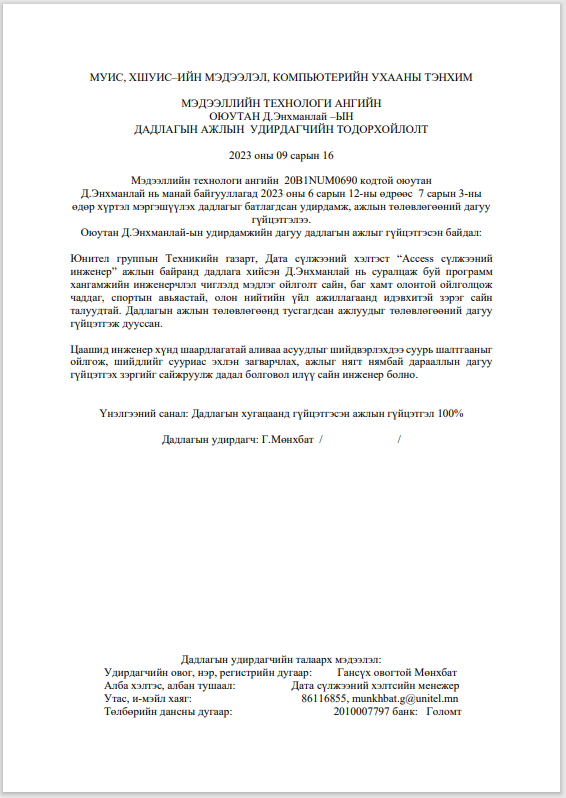
\includegraphics[width=14cm]{images/udirdamj.png}
% Хавсралтын нэр. Хавсралт гэдэг үг агуулахгүй

\end{document}
